\section{Modules}
\label{sec:Modules}
A Spring XD Module \cite{modules} is a unit of data processing and as mentioned above 
there are four types: source, processor, sink, and job. Modules in Spring XD are defined 
in their own application context. This allows for easy encapsulation and life cycle 
management for modules. Additionally, the use of an application context allows for easy 
module expansion.  Spring XD uses Spring Integration \cite{spring-integration-reference} 
as its foundation for implementing modules. A module is comprised of one or more channels 
and an integration bean.

\par

Spring XD offers a suite of 23 sources, 24 sinks, 9 processors and 9 jobs that are ready 
to use at startup.  These modules integrate with a variety of well
known and popular data stores and processing systems such as JDBC, HDFS, MongoDB, Spark,
and Sqoop.  If an existing module does not meet the needs of a given use case, Spring XD
supports custom modules.

Spring XD sink and source modules are Message Endpoints 
\cite{enterprise-integration-pattern-message-endpoint} 
that are responsible for sending data to and receiving data from external applications.
A source is the entry point for data into the stream. A sink is the module that dispatches
the stream's results to an external application or storage system. Batch jobs are used to
execute batch processing steps on a set of data.

\par

\subsection{Source}
Source modules receive inbound data and convert it to messages for
use by modules in a stream or by a batch job.
There are two source types: poller and event driven.  A poller source is based on the polling
consumer pattern \cite{enterprise-integration-pattern-pollingconsumer}. It
will poll an external application (such as a web service, FTP server, database) for data at a
configurable interval. An event driven source is based on the event driven
consumer pattern \cite{enterprise-integration-pattern-eventdrivenconsumer} which will
open a port to listen for incoming data that is pushed from an external application.

\par

In the case of a source module there is an ``output'' channel to dispatch messages 
transmitted by the bean to the stream (see figure~\ref{fig:sourcembc}.)

\par

\begin{figure}[ht]
\centering
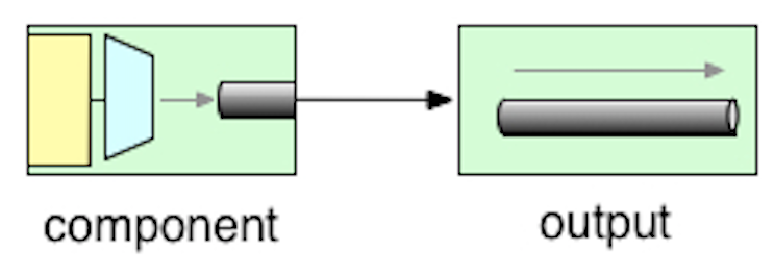
\epsfig{file=integration-module-output-channel.eps, height=.6in, width=1.75in}
\caption{Source Module Basic Components}
\label{fig:sourcembc}
\end{figure}

\par

\subsection{Processor}
A Processor module is used to modify the data as it passes on its way from the source to
the sink.  The basic processor is comprised of both an ``input'' and an ``output'' channel
and a bean.
The input channel receives all messages from the stream and dispatches
messages to the integration bean (see figure~\ref{fig:processormbc}.) It is the responsibility of
the bean to modify the data. The modified message is then sent to next module 
via the output channel.  

\par

\begin{figure}
\centering
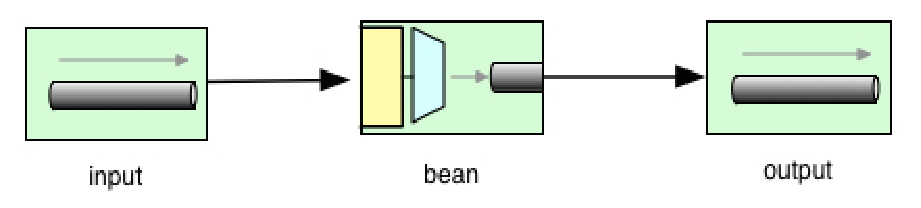
\epsfig{file=module-processor.eps, height=.6in, width=2.5in}
\caption{Processor Module Basic Components}
\label{fig:processormbc}
\end{figure}

\par

\subsection{Sink}
Sink modules convert and deliver messages from a stream in a format consumable by 
an external application.  There are two types of sinks: counter/gauge and delegate.
A counter/gauge is a specialized sink that increments a field on a data store every time a
message is received. (See section~\ref{sec:Analytics}.) A delegate
sink translates messages to the format expected by the external application.
After transforming the message, the resulting data is sent to the external application.

\par

The basic sink is comprised of a ``input'' channel and a bean.
The input channel receives all messages from the stream and dispatches
messages to the bean (see figure~\ref{fig:sinkmbc}.) It is the responsibility 
of the bean to implement retry behavior in cases of failure. The sinks 
included in Spring XD have configurable options for retries.

\par

\begin{figure}
\centering
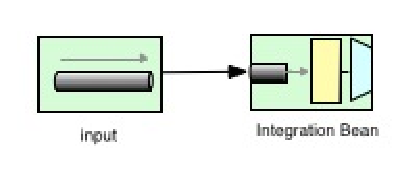
\epsfig{file=integration-module-input-channel.eps, height=.6in, width=1.75in}
\caption{Sink Module Basic Components}
\label{fig:sinkmbc}
\end{figure}

\par

\subsection{Job}
Spring XD uses Spring Batch \cite{spring-batch-reference} as the foundation for implementing
job modules. A job enables users to execute enterprise batch processes within Spring XD.
Jobs are typically used when running long lasting tasks that have transactional requirements.
To account for failure scenarios, the workflow in the job can be designed to restart and 
resume operation or roll-back the transaction altogether.

\par

A job is typically comprised of a job definition along with the supporting
bean(s) as shown in figure~\ref{fig:batchmbc}.
In some cases the job definition alone is sufficient to implement the desired behavior.

\par

\begin{figure}
\centering
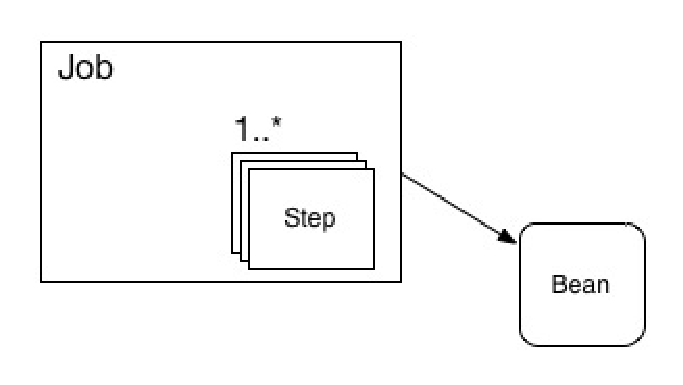
\epsfig{file=integration-batch.eps, height=.8in, width=2in}
\caption{Batch Basic Components}
\label{fig:batchmbc}
\end{figure}

\par 

\subsection{Deployment}
Modules are deployed in the modules directory and are segregated in
subdirectories by type: \texttt{modules/source}, \texttt{modules/processor}, 
\texttt{modules/sink} and \texttt{modules/job}.
These modules are dynamically loaded when a stream or job is deployed that requires that
specific module.

\par
\subsection{Composite}
A Composite module provides a way to create a single module 
comprised of other modules (processing chain).  A composite module can be used to prevent 
duplication when a processing chain of modules is used frequently.  
Performance is another reason to use composite modules, because messages between the 
modules that comprise the composite module will be transmitted in memory vs. the message 
bus.  

\par
